\section{Preventivo} \label{preventivo}

    Nella realizzazione del preventivo si è tenuto conto che, per i periodi di analisi e di analisi in dettaglio,
    le ore persona saranno di investimento e non a carico della \glossaryItem{Proponente}. Questo perché non esiste ancora un contratto
    tra la Proponente e il fornitore. Il contratto verrà stipulato con l'accettazione della proposta da parte della
    Proponente. \\
    La suddivisione delle ore tiene conto delle seguenti regole:

        \begin{enumerate}
            \item Ogni membro del gruppo dovrà sostenere circa la stessa mole di lavoro;
            \item Il totale delle ore sarà equamente distribuito tra i vari membri del gruppo;
            \item Possono esserci delle eccezioni per le regole precedenti, durante le sessioni d'esame.
            Coloro che non avranno esami da dare in tali periodi dovranno essere più disponibili per lavorare al progetto;
            \item Ogni membro del gruppo dovrà ricoprire ogni ruolo almeno una volta. È possibile che più di
            un membro, probabilmente tutti, ricopriranno più volte determinati ruoli durante il progetto;
            \item È importante che non si verifichino conflitti di interesse tra ruoli, ad esempio un Analista
            non deve verificare il proprio lavoro;
            \item In ogni periodo, ad eccezione dell'analisi in dettaglio, avverrà una rotazione di ruoli a
            circa metà periodo;
            \item Al termine di ogni periodo saranno assegnati nuovi ruoli;
            \item Se per una persona sono indicati due ruoli, significa che dovrà ricoprire tali ruoli sequenzialmente,
            nel periodo in cui gli sono stati assegnati.
        \end{enumerate}

    Per rendere le tabelle rappresentative del prospetto orario ed economico di ogni periodo facilmente leggibili,
    si utilizzano le seguenti abbreviazioni per i ruoli:

        \begin{itemize}
            \item \textbf{Resp}: Responsabile;
            \item \textbf{Admin}: Amministratore;
            \item \textbf{An}: Analista;
            \item \textbf{Proj}: Progettista;
            \item \textbf{Prog}: Programmatore;
            \item \textbf{Ver}: Verificatore.
        \end{itemize}

    Nelle varie tabelle, uno spazio vuoto significa che un determinato ruolo non è stato svolto da una determinata persona.
    Si ritiene che questo semplifichi la leggibilità delle tabelle.

\newpage

    \subsection{Analisi}

        \subsubsection{Rotazione ruoli}

            In questo periodo, la rotazione dei ruoli avviene in data 15 Dicembre 2017, secondo la seguente tabella:

            \begin{table}[htbp]
                \centering
                \begin{tabular}{| l | c | c |}
                \hline
                \centering
                &\multicolumn{2}{c |}{\textbf{Ruolo}}\\
                \hline
                \textbf{Membro} & \textbf{2017-11-10 - 2017-12-15} & \textbf{2017-12-16 - 2018-01-16}\\
                \hline
                \Tommaso & Admin & Resp\\
                \hline
                \Luca & Admin & Ver\\
                \hline
                \Mattia & Ver & An\\
                \hline
                \Leonardo & An & Ver\\
                \hline
                \Carlo & Ver & An\\
                \hline
                \Isacco & An & Ver\\
                \hline
                \Cristian & Resp & Ver\\
                \hline
                \end{tabular}
                \caption[Analisi - Rotazione ruoli]{Rotazione dei ruoli nell periodo di Analisi}
            \end{table}


            \subsubsection{Prospetto orario}

                Nel periodo di analisi, i membri del team ricoprono i seguenti ruoli con le rispettive ore associate: \\

                \begin{table}[htbp]
                    \centering
                    \begin{tabular}{| l | c  c c c c c c |}
                    \hline
                    \centering
                    \textbf{Nome} & \textbf{Admin} & \textbf{An} & \textbf{Proj} & \textbf{Prog} & \textbf{Resp} & \textbf{Ver} & \textbf{Totale} \\
                    \hline
                    \Tommaso & 12 & & & & 10 & & 22\\
                    \hline
                    \Luca & 13 & & & & & 5 & 18\\
                    \hline
                    \Mattia & & 15 & & & & 6 & 21\\
                    \hline
                    \Leonardo & & 15 & & & & 6 & 21\\
                    \hline
                    \Carlo & & 15 & & & & 6 & 21\\
                    \hline
                    \Isacco & & 15 & & & & 6 & 21\\
                    \hline
                    \Cristian & & & & & 10 & 6 & 16\\
                    \hline
                    \end{tabular}
                    \caption[Analisi - Distribuzione oraria]{Distribuzione oraria nel periodo di Analisi}
                \end{table}

\newpage

                Il seguente istogramma fornisce una rappresentazione visiva della suddivisione oraria:

                    \begin{figure}[htbp]
                    	\centering
                        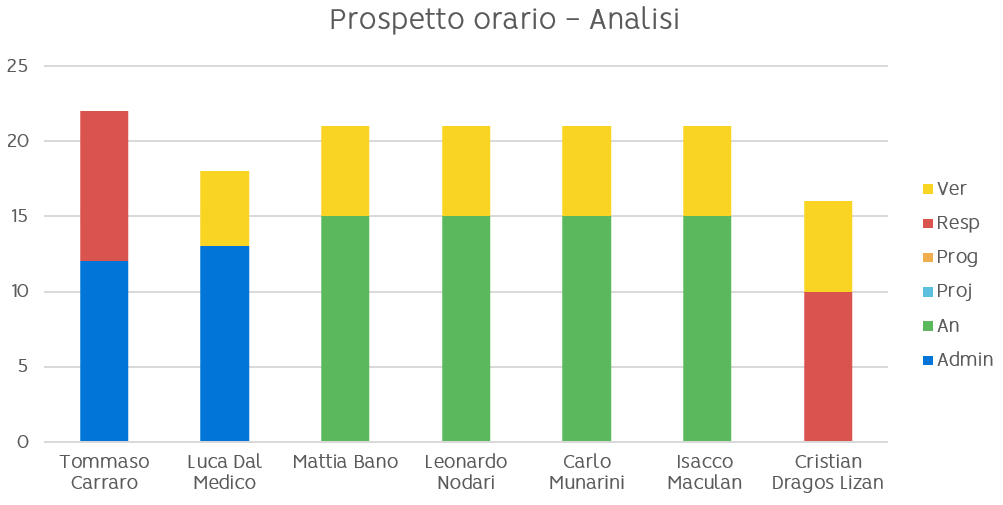
\includegraphics[width=14cm,height=14cm,keepaspectratio]{./img/ProspettoOrario/POAnalisi.png}
                        \caption[Analisi - Istogramma prospetto orario]{Istogramma del prospetto orario per il periodo di analisi}
                    \end{figure}
                

            \subsubsection{Prospetto economico}

                Nel periodo di analisi, la distribuzione delle ore, con rispettivo costo tra i differenti ruoli, è la seguente:

                \begin{table}[htbp]
                    \centering
                    \begin{tabular}{| l c c |}
                        \hline
                        \textbf{Ruolo} & \textbf{Ore} & \textbf{Costo in €}\\
                        \hline
                        Amministratore & 25 & 500.00\\
                        Analista & 60 & 1500.00\\
                        Progettista & & \\
                        Programmatore & & \\
                        Responsabile & 20 & 600.00\\
                        Verificatore & 35 & 525.00\\
                        \hline
                        \textbf{Totale} & \textbf{140} & \textbf{3125.00}\\
                        \hline
                    \end{tabular}
                    \caption[Analisi - Prospetto economico]{Prospetto economico nel periodo di Analisi}
                \end{table}

\newpage

                Il seguente diagramma a torta fornisce una rappresentazione visiva della distribuzione dei ruoli nel periodo di analisi:

                
                    \begin{figure}[htbp]
                    	\centering
                        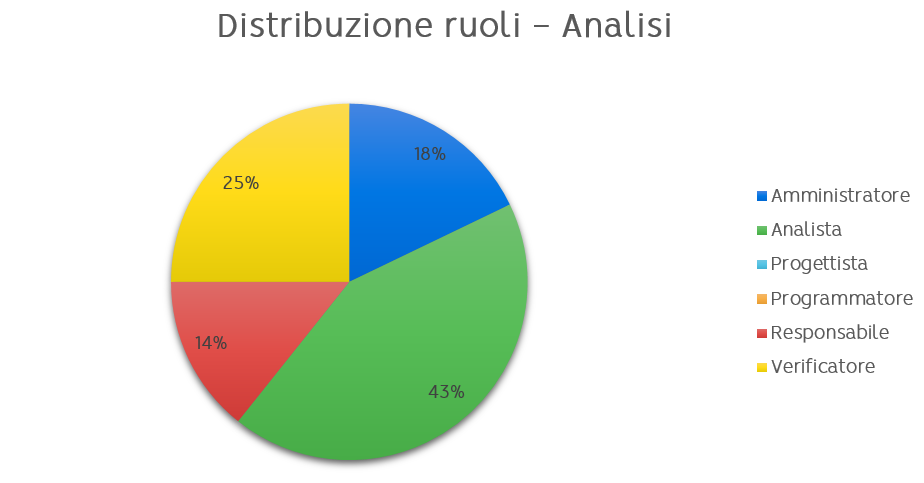
\includegraphics[width=14cm,height=14cm,keepaspectratio]{./img/ProspettoOrario/SRAnalisi.png}
                        \caption[Analisi - Diagramma a torta suddivisione ruoli]{Diagramma a torta della distribuzione dei ruoli nel periodo di analisi}
                    \end{figure}
                

\newpage

    \subsection{Analisi in dettaglio}

        \subsubsection{Rotazione ruoli}

            In questo periodo, non vi è rotazione dei ruoli, perché di durata insufficiente per una rotazione efficace.

        \subsubsection{Prospetto orario}

            Nel periodo di analisi in dettaglio, i membri del team ricoprono i seguenti ruoli con le rispettive ore associate: \\


            \begin{table}[htbp]
                \centering
                    \begin{tabular}{| l | c  c c c c c c |}
                        \hline
                        \centering
                        \textbf{Nome} & \textbf{Admin} & \textbf{An} & \textbf{Proj} & \textbf{Prog} & \textbf{Resp} & \textbf{Ver} & \textbf{Totale} \\
                        \hline
                        \Tommaso & & & & & & 7 & 7\\
                        \hline
                        \Luca & & 10 & & & & & 10\\
                        \hline
                        \Mattia & & & & & & 7 & 7\\
                        \hline
                        \Leonardo & 4 & & & & 5 & & 9\\
                        \hline
                        \Carlo & & & & & & 8 & 8\\
                        \hline
                        \Isacco & & & & & & 8 & 8\\
                        \hline
                        \Cristian & 11 & & & & & & 11\\
                        \hline
                    \end{tabular}
                \caption[Analisi in dettaglio - Distribuzione oraria]{Distribuzione oraria nel periodo di Analisi in Dettaglio}
            \end{table}

            Il seguente istogramma fornisce una rappresentazione visiva della suddivisione oraria:

            
                \begin{figure}[htbp]
                	\centering
                    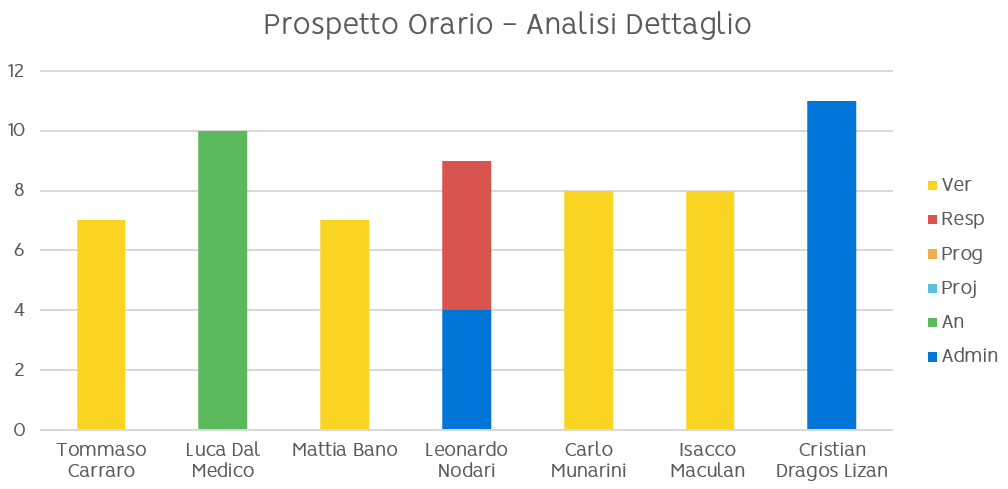
\includegraphics[width=14cm,height=14cm,keepaspectratio]{./img/ProspettoOrario/POAnalisiDettaglio.png}
                    \caption[Analisi dettaglio - Istogramma prospetto orario]{Istogramma del prospetto orario per il periodo di analisi in dettaglio}
                \end{figure}
            

        \subsubsection{Prospetto economico}

            Nel periodo di analisi in dettaglio, la distribuzione delle ore, con rispettivo costo tra i differenti ruoli,
            è la seguente:

            \begin{table}[htbp]
                \centering
                    \begin{tabular}{| l c c |}
                        \hline
                        \textbf{Ruolo} & \textbf{Ore} & \textbf{Costo in €}\\
                        \hline
                        Amministratore & 15 & 300.00\\
                        Analista & 10 & 250.00\\
                        Progettista & & \\
                        Programmatore & & \\
                        Responsabile & 5 & 150.00\\
                        Verificatore & 30 & 450.00\\
                        \hline
                        \textbf{Totale} & \textbf{60} & \textbf{1150.00}\\
                        \hline
                    \end{tabular}
                \caption[Analisi in dettaglio - Prospetto economico]{Prospetto economico nel periodo di Analisi in Dettaglio}
            \end{table}

Il seguente diagramma a torta fornisce una rappresentazione visiva della distribuzione dei ruoli nel periodo di analisi in dettaglio:

\begin{figure}[htbp]
\centering
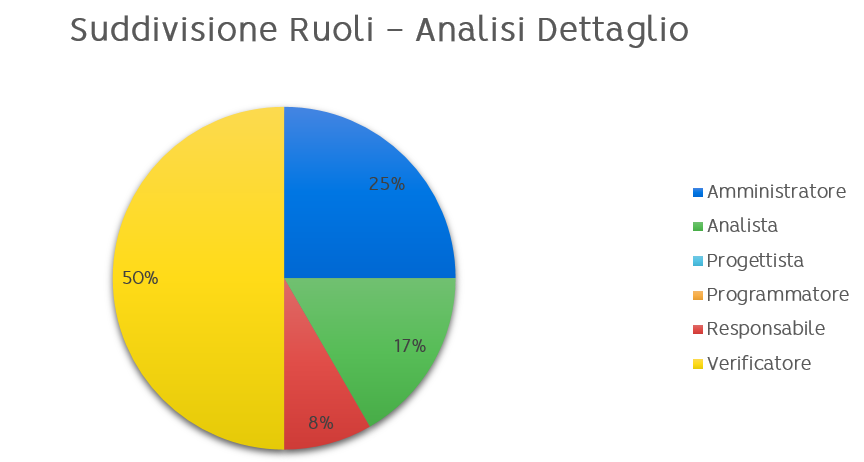
\includegraphics[width=14cm,height=14cm,keepaspectratio]{./img/ProspettoOrario/SRAnalisiDettaglio.png}
\caption[Analisi dettaglio - Diagramma a torta suddivisione ruoli]{Diagramma a torta della distribuzione dei ruoli nel periodo di analisi in dettaglio}
\end{figure}

\newpage

\subsection{Progettazione architetturale}
\subsubsection{Rotazione ruoli}
In questo periodo, la rotazione dei ruoli avviene in data 23 Febbraio 2017, secondo la seguente tabella:

\begin{table}[htbp]
\centering
\begin{tabular}{| l | c | c |}
\hline
\centering
&\multicolumn{2}{c |}{\textbf{Ruolo}}\\
\hline
\textbf{Membro} & \textbf{2018-01-27 - 2018-02-23} & \textbf{2018-02-24 - 2018-03-19}\\
\hline
\Tommaso & An/Proj & Prog\\
\hline
\Luca & Proj & Resp\\
\hline
\Mattia & Admin & Ver\\
\hline
\Leonardo & Resp/Proj & Prog\\
\hline
\Carlo & Ver & An/Proj\\
\hline
\Isacco & Proj & Ver\\
\hline
\Cristian & Ver/Proj & Prog\\
\hline
\end{tabular}
\caption[Progettazione architetturale - Rotazione ruoli]{Rotazione dei ruoli nel periodo di Progettazione Architetturale}
\end{table}

\subsubsection{Prospetto orario}
Nel periodo di progettazione architetturale, i membri del team ricoprono i seguenti ruoli con le rispettive ore associate:\\


\begin{table}[htbp]
\centering
\begin{tabular}{| l | c  c c c c c c |}
\hline
\centering
\textbf{Nome} & \textbf{Admin} & \textbf{An} & \textbf{Proj} & \textbf{Prog} & \textbf{Resp} & \textbf{Ver} & \textbf{Totale} \\
\hline
\Tommaso & & 10 & 15 & 10 & & & 35\\
\hline
\Luca & & & 26 & & 10 & & 36\\
\hline
\Mattia & 15 & & & & & 20 & 35\\
\hline
\Leonardo & & & 15 & 17 & 5 & & 37\\
\hline
\Carlo & & & 16 & & & 20 & 36\\
\hline
\Isacco & & & 17 & & & 20 & 37\\
\hline
\Cristian & & & 15 & 15 & & 10 & 40\\
\hline
\end{tabular}
\caption[Progettazione architetturale - Distribuzione oraria]{Distribuzione oraria nel periodo di Progettazione Architetturale}
\end{table}
\newpage
Il seguente istogramma fornisce una rappresentazione visiva della suddivisione oraria:

\begin{figure}[htbp]
\centering
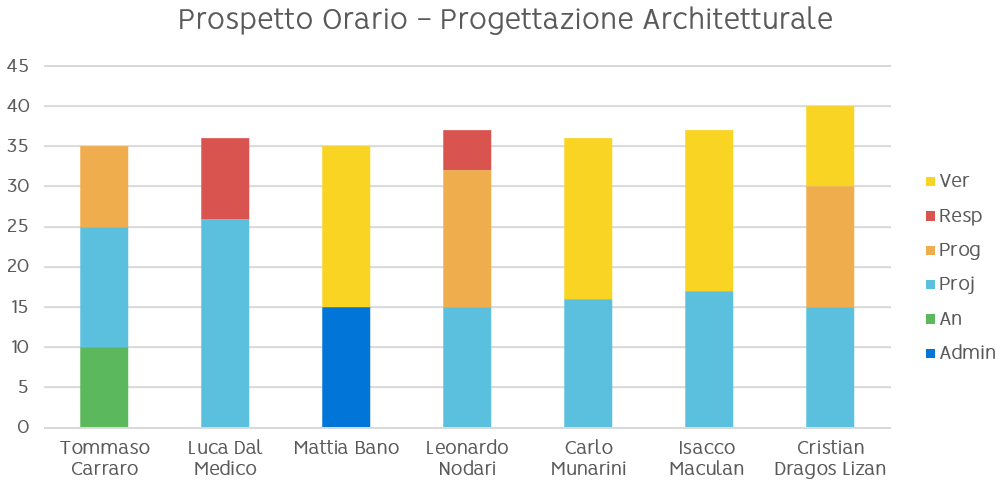
\includegraphics[width=14cm,height=14cm,keepaspectratio]{./img/ProspettoOrario/POProgArch.png}
\caption[Progettazione architetturale - Istogramma prospetto orario]{Istogramma del prospetto orario per il periodo di progettazione architetturale}
\end{figure}


\subsubsection{Prospetto economico}
Nel periodo di progettazione architetturale, la distribuzione delle ore, con rispettivo costo tra i differenti ruoli, è la seguente:

\begin{table}[htbp]
\centering
\begin{tabular}{| l c c |}
\hline
\textbf{Ruolo} & \textbf{Ore} & \textbf{Costo in €}\\
\hline
Amministratore & 15 & 300.00\\
Analista & 10 & 250.00\\
Progettista & 104 & 2288.00 \\
Programmatore & 42 & 630.00\\
Responsabile & 15 & 450.00\\
Verificatore & 70 & 1050.00\\
\hline
\textbf{Totale} & \textbf{256} & \textbf{4968.00}\\
\hline
\end{tabular}
\caption[Progettazione architetturale - Prospetto economico]{Prospetto economico nel periodo di Progettazione Architetturale}
\end{table}
\newpage
Il seguente diagramma a torta fornisce una rappresentazione visiva della distribuzione dei ruoli nel periodo di progettazione architetturale:

\begin{figure}[htbp]
\centering
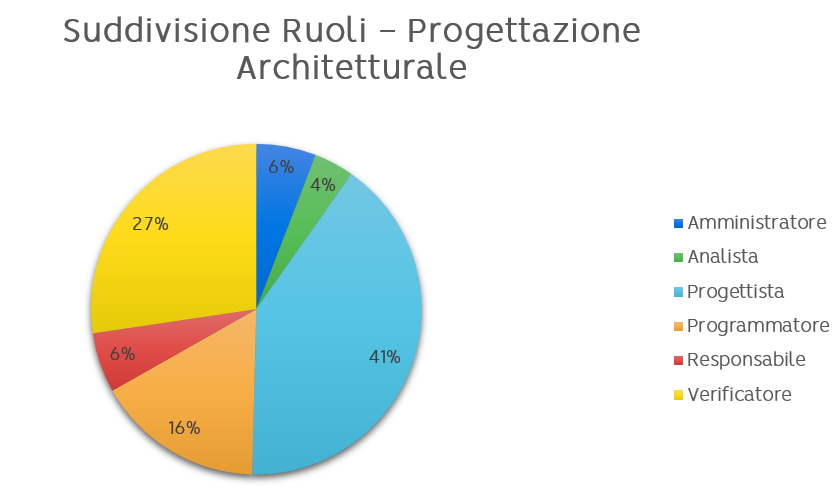
\includegraphics[width=14cm,height=14cm,keepaspectratio]{./img/ProspettoOrario/SRProgArch.png}
\caption[Progettazione architetturale - Diagramma a torta suddivisione ruoli]{Diagramma a torta della distribuzione dei ruoli nel periodo di progettazione architetturale}
\end{figure}

\newpage

\subsection{Progettazione in dettaglio e codifica}
\subsubsection{Rotazione ruoli}
Per questo periodo è stata fatta una ripianificazione. I motivi sono spiegati nel verbale interno del 5 Aprile 2018 e in sezione §\ref{inSeguitoRP}.
La rotazione dei ruoli avviene in data 23 Aprile 2018, secondo la seguente tabella:

\begin{table}[htbp]
\centering
\begin{tabular}{| l | c | c |}
\hline
\centering
&\multicolumn{2}{c |}{\textbf{Ruolo}}\\
\hline
\textbf{Membro} & \textbf{2018-03-20 - 2018-04-23} & \textbf{2018-04-24 - 2018-05-14}\\
\hline
\Tommaso & An/Proj & Ver\\
\hline
\Luca & Proj & Prog/Ver\\
\hline
\Mattia & Proj/Resp & Prog\\
\hline
\Leonardo & Proj/Ver & Ver\\
\hline
\Carlo & Admin & Prog/Ver\\
\hline
\Isacco & Admin/Ver & Prog/Resp\\
\hline
\Cristian & An/Proj & Ver\\
\hline
\end{tabular}
\caption[Progettazione in dettaglio e codifica - Rotazione ruoli]{Rotazione dei ruoli nel periodo di Progettazione in Dettaglio e Codifica}
\end{table}

\subsubsection{Prospetto orario}
Nel periodo di progettazione in dettaglio e codifica, i membri del team ricoprono i seguenti ruoli con le rispettive ore associate:\\

\begin{table}[htbp]
\centering
\begin{tabular}{| l | c  c c c c c c |}
\hline
\centering
\textbf{Nome} & \textbf{Admin} & \textbf{An} & \textbf{Proj} & \textbf{Prog} & \textbf{Resp} & \textbf{Ver} & \textbf{Totale} \\
\hline
\Tommaso & & 3 & 15 & & & 35 & 53\\
\hline
\Luca & & & 15 & 28 & & 8 & 51\\
\hline
\Mattia & & & 20 & 22 & 10 & & 52\\
\hline
\Leonardo & & & 20 & & & 25 & 45\\
\hline
\Carlo & 8 & & & 25 & & 12 & 45\\
\hline
\Isacco & 12 & & & 25 & 5 & 8 & 50\\
\hline
\Cristian & & 7 & 30 & & & 7 & 44\\
\hline
\end{tabular}
\caption[Progettazione in dettaglio e codifica - Distribuzione oraria]{Distribuzione oraria nel periodo di Progettazione in Dettaglio e Codifica}
\end{table}
\newpage
Il seguente istogramma fornisce una rappresentazione visiva della suddivisione oraria:

\begin{figure}[htbp]
\centering
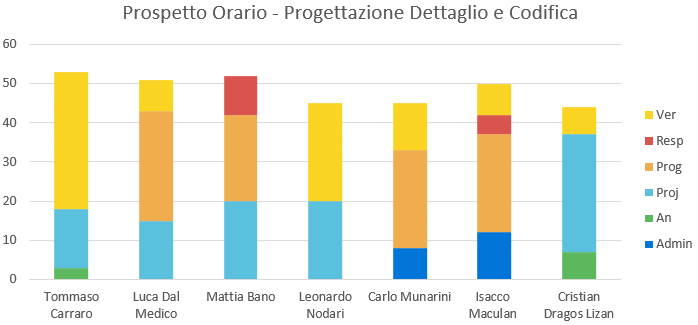
\includegraphics[width=14cm,height=14cm,keepaspectratio]{./img/ProspettoOrario/POProgDettCod.png}
\caption[Progettazione dettaglio e codifica - Istogramma prospetto orario]{Istogramma del prospetto orario per il periodo di progettazione in dettaglio e codifica}
\end{figure}


\subsubsection{Prospetto economico}
Nel periodo di progettazione in dettaglio e codifica, la distribuzione delle ore, con rispettivo costo tra i differenti ruoli, è la seguente:

\begin{table}[htbp]
\centering
\begin{tabular}{| l c c |}
\hline
\textbf{Ruolo} & \textbf{Ore} & \textbf{Costo in €}\\
\hline
Amministratore & 20 & 400.00\\
Analista & 10 & 250.00\\
Progettista & 100 & 2200.00 \\
Programmatore & 100 & 1500.00\\
Responsabile & 15 & 450.00\\
Verificatore & 95 & 1425.00\\
\hline
\textbf{Totale} & \textbf{340} & \textbf{6225.00}\\
\hline
\end{tabular}
\caption[Progettazione in dettaglio e codifica - Prospetto economico]{Prospetto economico nel periodo di Progettazione in Dettaglio e Codifica}
\end{table}
\newpage
Il seguente diagramma a torta fornisce una rappresentazione visiva della distribuzione dei ruoli nel periodo di progettazione in dettaglio e codifica:

\begin{figure}[htbp]
\centering
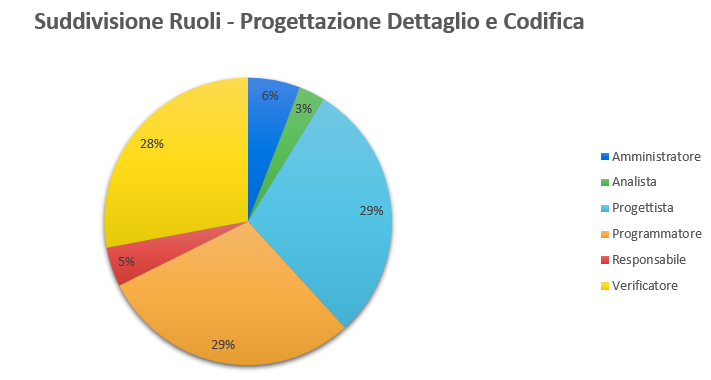
\includegraphics[width=14cm,height=14cm,keepaspectratio]{./img/ProspettoOrario/SRProgDettCod.png}
\caption[Progettazione dettaglio e codifica - Diagramma a torta suddivisione ruoli]{Diagramma a torta della distribuzione dei ruoli nel periodo di progettazione in dettaglio e codifica}
\end{figure}

\newpage

\subsection{Validazione e collaudo}
\subsubsection{Rotazione ruoli}
Per questo periodo è stata fatta una ripianificazione. I motivi sono spiegati nel verbale interno del 5 Aprile 2018.
La rotazione dei ruoli avviene in data 1 Giugno 2018, secondo la seguente tabella:

\begin{table}[htbp]
\centering
\begin{tabular}{| l | c | c |}
\hline
\centering
&\multicolumn{2}{c |}{\textbf{Ruolo}}\\
\hline
\textbf{Membro} & \textbf{2018-05-15 - 2018-06-01} & \textbf{2018-06-02 - 2018-06-15}\\
\hline
\Tommaso & Prog &\\
\hline
\Luca & & Ver\\
\hline
\Mattia & Proj & Ver\\
\hline
\Leonardo & Admin & Ver\\
\hline
\Carlo & Resp/Admin & Ver\\
\hline
\Isacco & Proj/Ver & Resp\\
\hline
\Cristian & Prog & Ver\\
\hline
\end{tabular}
\caption[Validazione e collaudo - Rotazione ruoli]{Rotazione dei ruoli nel periodo di Validazione e Collaudo}
\end{table}

\subsubsection{Prospetto orario}
Nel periodo di validazione e collaudo, i membri del team ricoprono i seguenti ruoli con le rispettive ore associate:\\

\begin{table}[htbp]
\centering
\begin{tabular}{| l | c  c c c c c c |}
\hline
\centering
\textbf{Nome} & \textbf{Admin} & \textbf{An} & \textbf{Proj} & \textbf{Prog} & \textbf{Resp} & \textbf{Ver} & \textbf{Totale} \\
\hline
\Tommaso & & & & 15 & & & 15\\
\hline
\Luca & & & & & & 16 & 16\\
\hline
\Mattia & & & 9 & & & 7 & 16\\
\hline
\Leonardo & 10 & & & & & 11 & 21\\
\hline
\Carlo & 5 & & & & 10 & 7 & 22\\
\hline
\Isacco & & & 11 & & 5 & & 16\\
\hline
\Cristian & & & & 5 & & 14 & 19\\
\hline
\end{tabular}
\caption[Validazione e collaudo - Distribuzione oraria]{Distribuzione oraria nel periodo di Validazione e Collaudo}
\end{table}
\newpage
Il seguente istogramma fornisce una rappresentazione visiva della suddivisione oraria:

\begin{figure}[htbp]
\centering
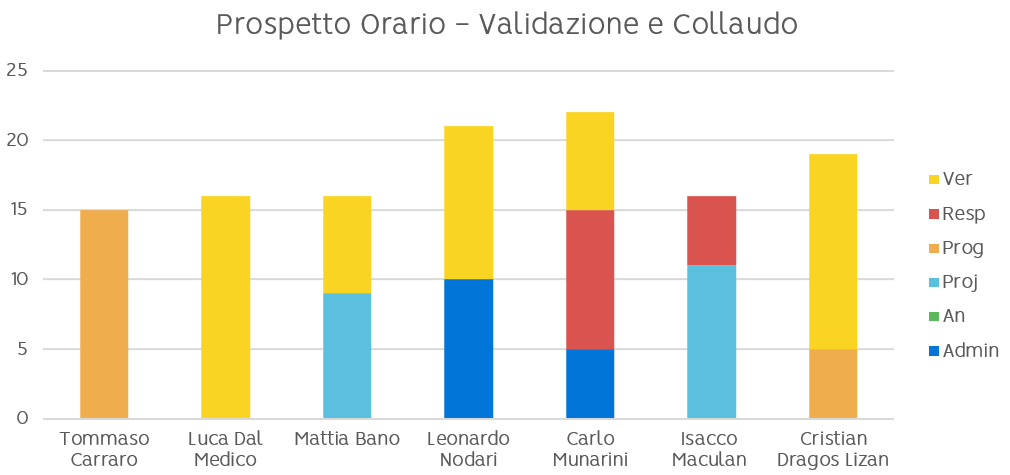
\includegraphics[width=14cm,height=14cm,keepaspectratio]{./img/ProspettoOrario/POValidazioneCollaudo.png}
\caption[Validazione e collaudo - Istogramma prospetto orario]{Istogramma del prospetto orario per il periodo di validazione e collaudo}
\end{figure}


\subsubsection{Prospetto economico}
Nel periodo di validazione e collaudo, la distribuzione delle ore, con rispettivo costo tra i differenti ruoli, è la seguente:

\begin{table}[htbp]
\centering
\begin{tabular}{| l c c |}
\hline
\textbf{Ruolo} & \textbf{Ore} & \textbf{Costo in €}\\
\hline
Amministratore & 15 & 300.00\\
Analista &  & \\
Progettista & 20 & 440.00 \\
Programmatore & 20 & 300.00\\
Responsabile & 15 & 450.00\\
Verificatore & 55 & 825.00\\
\hline
\textbf{Totale} & \textbf{125} & \textbf{2315.00}\\
\hline
\end{tabular}
\caption[Validazione e collaudo - Prospetto economico]{Prospetto economico nel periodo di Validazione e Collaudo}
\end{table}
\newpage
Il seguente diagramma a torta fornisce una rappresentazione visiva della distribuzione dei ruoli nel periodo di validazione e collaudo:

\begin{figure}[htbp]
\centering
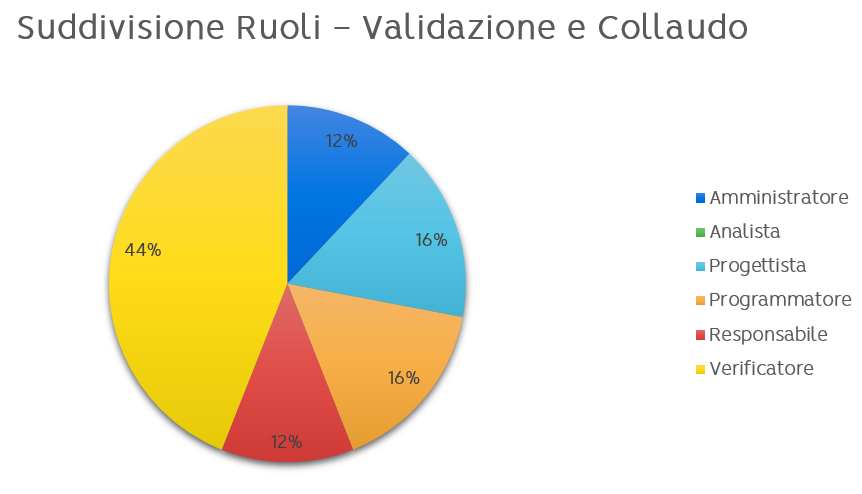
\includegraphics[width=14cm,height=14cm,keepaspectratio]{./img/ProspettoOrario/SRValidazioneCollaudo.png}
\caption[Validazione e collaudo - Diagramma a torta suddivisione ruoli]{Diagramma a torta della distribuzione dei ruoli nel periodo di validazione e collaudo}
\end{figure}

\newpage

\subsection{Totale}
\subsubsection{Prospetto orario totale con investimento}
Nella seguente tabella è riportata la distribuzione delle ore totali, rendicontate e di investimento, per lo svolgimento
dell'intero progetto. Le ore di investimento sono principalmente collocate nei primi periodi del progetto, in quanto
non esiste ancora un contratto con la Proponente.

\begin{table}[htbp]
\centering
\begin{tabular}{| l | c  c c c c c c |}
\hline
\centering
\textbf{Nome} & \textbf{Admin} & \textbf{An} & \textbf{Proj} & \textbf{Prog} & \textbf{Resp} & \textbf{Ver} & \textbf{Totale} \\
\hline
\Tommaso & 12 & 13 & 30 & 25 & 10 & 42 & 132\\
\hline
\Luca & 13 & 10 & 41 & 28 & 10 & 29 & 131\\
\hline
\Mattia & 15 & 15 & 29 & 22 & 10 & 40 & 131\\
\hline
\Leonardo & 14 & 15 & 35 & 17 & 10 & 42 & 133\\
\hline
\Carlo & 13 & 15 & 16 & 25 & 10 & 53 & 132\\
\hline
\Isacco & 12 & 15 & 28 & 25 & 10 & 42 & 132\\
\hline
\Cristian & 11 & 7 & 45 & 20 & 10 & 37 & 130\\
\hline
\end{tabular}
\caption[Totale con investimento - Distribuzione oraria]{Distribuzione oraria totale con investimento}
\end{table}

Il seguente istogramma fornisce una rappresentazione visiva della suddivisione oraria totale con ore di investimento:

\begin{figure}[htbp]
\centering
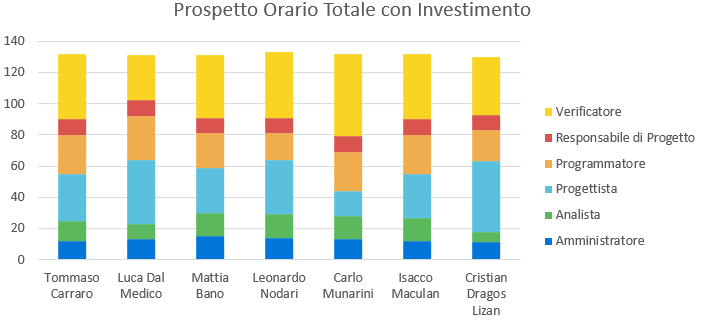
\includegraphics[width=14cm,height=14cm,keepaspectratio]{./img/ProspettoOrario/POTotInv.png}
\caption[Totale con investimento - Istogramma prospetto orario]{Istogramma del prospetto orario totale con ore di investimento}
\end{figure}


\subsubsection{Prospetto economico totale con investimento}
La distribuzione delle ore con investimento, con rispettivo costo tra i differenti ruoli, è la seguente:

\begin{table}[htbp]
\centering
\begin{tabular}{| l c c |}
\hline
\textbf{Ruolo} & \textbf{Ore} & \textbf{Costo in €}\\
\hline
Amministratore & 90 & 1800.00\\
Analista & 90 & 2250.00 \\
Progettista & 224 & 4928.00 \\
Programmatore & 162 & 2430.00\\
Responsabile & 70 & 2100.00\\
Verificatore & 285 & 4275.00\\
\hline
\textbf{Totale} & \textbf{921} & \textbf{17783.00}\\
\hline
\end{tabular}
\caption[Totale con investimento - Prospetto economico]{Prospetto economico totale con investimento}
\end{table}

Il seguente diagramma a torta fornisce una rappresentazione visiva della distribuzione dei ruoli, comprese le ore con investimento, nell'intera durata del progetto:

\begin{figure}[htbp]
\centering
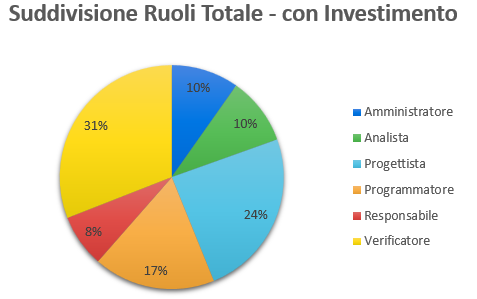
\includegraphics[width=14cm,height=14cm,keepaspectratio]{./img/ProspettoOrario/SRTotInv.png}
\caption[Totale con investimento - Diagramma a torta suddivisione ruoli]{Diagramma a torta della distribuzione totale dei ruoli con ore di investimento}
\end{figure}

\newpage

\subsubsection{Prospetto orario totale con ore rendicontate}
Nella seguente tabella è riportata la distribuzione delle ore totali rendicontate per lo svolgimento dell'intero progetto.
\begin{table}[htbp]
\centering
\begin{tabular}{| l | c  c c c c c c |}
\hline
\centering
\textbf{Nome} & \textbf{Admin} & \textbf{An} & \textbf{Proj} & \textbf{Prog} & \textbf{Resp} & \textbf{Ver} & \textbf{Totale} \\
\hline
\Tommaso & & 13 & 30 & 25 &  & 35 & 103\\
\hline
\Luca & & & 41 & 28 & 10 & 24 & 103\\
\hline
\Mattia & 15 & & 29 & 22 & 10 & 27 & 103\\
\hline
\Leonardo & 10 & & 35 & 17 & 5 & 36 & 103\\
\hline
\Carlo & 13 & & 16 & 25 & 10 & 39 & 103\\
\hline
\Isacco & 12 & & 28 & 25 & 10 & 28 & 103\\
\hline
\Cristian & & 7 & 45 & 20 & & 31 & 103\\
\hline
\end{tabular}
\caption[Totale con ore rendicontate - Distribuzione oraria]{Distribuzione oraria totale con ore rendicontate}
\end{table}

Il seguente istogramma fornisce una rappresentazione visiva della suddivisione oraria totale con ore rendicontate:

\begin{figure}[htbp]
\centering
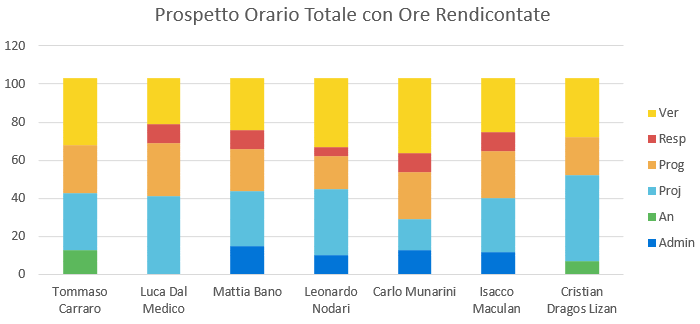
\includegraphics[width=14cm,height=14cm,keepaspectratio]{./img/ProspettoOrario/POTotRend.png}
\caption[Totale con ore rendicontate - Istogramma prospetto orario]{Istogramma del prospetto orario totale con ore rendicontate}
\end{figure}

\newpage

\subsubsection{Prospetto economico totale con ore rendicontate}
La distribuzione delle ore rendicontate, con rispettivo costo tra i differenti ruoli, è la seguente:

\begin{table}[htbp]
\centering
\begin{tabular}{| l c c |}
\hline
\textbf{Ruolo} & \textbf{Ore} & \textbf{Costo in €}\\
\hline
Amministratore & 50 & 1000.00\\
Analista & 20 & 500.00 \\
Progettista & 224 & 4928.00 \\
Programmatore & 162 & 2430.00\\
Responsabile & 45 & 1350.00\\
Verificatore & 220 & 3300.00\\
\hline
\textbf{Totale} & \textbf{723} & \textbf{13508.00}\\
\hline
\end{tabular}
\caption[Totale con ore rendicontate - Prospetto economico]{Prospetto economico totale con ore rendicontate}
\end{table}

Il seguente diagramma a torta fornisce una rappresentazione visiva della distribuzione dei ruoli, escluse le ore di investimento, nell'intera durata del progetto:

\begin{figure}[htbp]
\centering
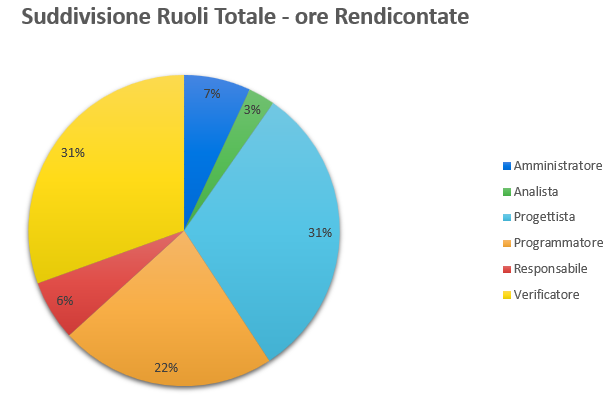
\includegraphics[width=14cm,height=14cm,keepaspectratio]{./img/ProspettoOrario/SRTotRend.png}
\caption[Totale con ore rendicontate - Diagramma a torta suddivisione ruoli]{Diagramma a torta della distribuzione totale dei ruoli con ore rendicontate}
\end{figure}

\newpage

\section{Consuntivo e preventivo a finire}
In questa sezione vengono presentati i consuntivi dei vari periodi con una breve valutazione degli stessi. Al termine della sezione verrà presentato un preventivo a finire che terrà conto dei soli periodi rendicontati. Verranno presentati i consuntivi dei soli periodi rendicontati, ovvero i periodi che si collocano dopo il superamento della revisione dei requisiti. I valori presentati saranno:
\begin{itemize}
\item \textbf{Positivi}: se il valore del preventivo è superiore al valore del consuntivo e quindi è stato necessario meno tempo persona del previsto;
\item \textbf{Negativi}: se il valore del preventivo è inferiore al valore del consuntivo e quindi è stato necessario più tempo persona del previsto.
\end{itemize}
\subsection{Periodo di progettazione architetturale}
\subsubsection{Consuntivo} \label{consuntivo1}
La seguente tabella mostra i dati del consuntivo per il periodo di progettazione architetturale.

\begin{table}[htbp]
\centering
\begin{tabular}{| l | c  c | c c |}
\hline
&\multicolumn{2}{c |}{\textbf{Ore}} & \multicolumn{2}{c |}{\textbf{Costo in €}}\\
\hline
\textbf{Ruolo} & \textbf{Preventivo} & \textbf{Consuntivo} & \textbf{Preventivo} & \textbf{Consuntivo}\\
\hline
Amministratore & 15 & 15 & 300.00 & 300.00\\
Analista & 10 & 30(-20) & 250.00 & 750.00(-500.00)\\
Progettista & 104 & 70(+34) & 2288.00 & 1540.00(+748.00)\\
Programmatore & 42 & 35(+7) & 630.00 & 525.00(+105.00)\\
Responsabile & 15 & 25(-10) & 450.00 & 750.00(-300.00)\\
Verificatore & 70 & 70 & 1050.00 & 1050.00\\
\hline
\textbf{Totale} & \textbf{256} & \textbf{245} & \textbf{4968.00} & \textbf{4915.00} \\
\hline
\textbf{Differenza} & \multicolumn{2}{c |}{\textbf{+11 Ore}} & \multicolumn{2}{c |}{\textbf{(+53.00)€}}\\
\hline
\end{tabular}
\caption[Progettazione architetturale - Consuntivo]{Prospetto orario ed economico a consuntivo del periodo di progettazione architetturale}
\end{table}

\subsubsection{Conclusione}
Durante il periodo di progettazione architetturale sono state utilizzate più ore dei seguenti ruoli:
\begin{itemize}
	\item Analista;
	\item Responsabile di progetto.
\end{itemize} 
L'incremento delle ore di Analista e Responsabile è dovuto ad una sottostima del carico di lavoro per l'incremento dell'\AnalisiRequisiti{}, del \PianoProgetto{} e del \PianoQualifica{}. All'interno di questi documenti, in particolare, sono state segnalate delle lacune dai Committenti, quando il team non si aspettava la presenza di tali errori.\\
Al contempo, si è riscontrato un risparmio delle ore dedicate a:
\begin{itemize}
	\item Progettista;
	\item Programmatore.
\end{itemize}
Questo è stato dovuto ad una sovrastima data da una cattiva comprensione da parte dei componenti del gruppo dei concetti di Technology Baseline e Proof of Concept. Si pensava infatti che la Technology Baseline richiedesse molte ore di progettazione ma dopo uno studio e un'analisi più in dettaglio si è scoperto che si trattava di un semi-elaborato contenente le scelte tecnologiche fatte.\\
Il lavoro del Progettista sarà tuttavia richiesto nel periodo successivo per la stesura della Product Baseline che invece richiede progettazione, anche tramite diagrammi di classe e di sequenza. Per quanto riguarda le ore di Verificatore, queste sono state sufficienti per verificare tutti i documenti incrementati in questo periodo.\\
In conclusione il gruppo ha risparmiato in tutto 11 ore e 53.00 € nel periodo di progettazione architetturale.
\newpage
\subsection{Periodo di progettazione in dettaglio e codifica}
\subsubsection{Consuntivo} \label{consuntivo2}
La seguente tabella mostra i dati del consuntivo per il periodo di progettazione in dettaglio e codifica.

\begin{table}[htbp]
\centering
\begin{tabular}{| l | c  c | c c |}
\hline
&\multicolumn{2}{c |}{\textbf{Ore}} & \multicolumn{2}{c |}{\textbf{Costo in €}}\\
\hline
\textbf{Ruolo} & \textbf{Preventivo} & \textbf{Consuntivo} & \textbf{Preventivo} & \textbf{Consuntivo}\\
\hline
Amministratore & 20 & 20 & 400.00 & 400.00\\
Analista & 10 & 12(-2) & 250.00 & 300.00(-50.00)\\
Progettista & 100 & 100 & 2200.00 & 2200.00\\
Programmatore & 100 & 96(+4) & 1500.00 & 1440.00(+60.00)\\
Responsabile & 15 & 15 & 450.00 & 450.00\\
Verificatore & 95 & 95 & 1425.00 & 1425.00\\
\hline
\textbf{Totale} & \textbf{340} & \textbf{338} & \textbf{6225.00} & \textbf{6215.00} \\
\hline
\textbf{Differenza} & \multicolumn{2}{c |}{\textbf{+2 Ore}} & \multicolumn{2}{c |}{\textbf{(+10.00)€}}\\
\hline
\end{tabular}
\caption[Progettazione in dettaglio e codifica - Consuntivo]{Prospetto orario ed economico a consuntivo del periodo di progettazione in dettaglio e codifica}
\end{table}

\subsubsection{Conclusione}
Nel periodo di progettazione in dettaglio e codifica sono servite due ore in più del previsto per il ruolo di Analista. Infatti nella valutazione della revisione di progettazione ci sono stati ulteriori problemi nel documento Analisi dei Requisiti. 12 ore sono bastate per cambiare la struttura del documento ed effettuare le modifiche richieste dal \glossaryItem{Committente} per casi d'uso e vincoli. In particolare è stato richiesto di  chiarire definitivamente le funzionalità offerte dal sistema agli attori esterni. Inizialmente erano 10 le ore di Analista pianificate, ma sono stati investiti 50.00 € dei soldi risparmiati in seguito alla revisione di progettazione. \\
La codifica del prodotto ha richiesto 4 ore in meno di Programmatore con un risparmio di 60.00 €. Queste ore saranno utilizzate all'occorrenza in preparazione alla revisione di accettazione nel caso siano necessari ultimi ritocchi o correzioni di bug.\\
Per concludere, in questo periodo, sono state risparmiate due ore e 10.00 € in totale.
\newpage

\subsection{Periodo di validazione e collaudo}
\subsubsection{Consuntivo} \label{consuntivo3}
La seguente tabella mostra i dati del consuntivo per il periodo di validazione e collaudo.

\begin{table}[htbp]
\centering
\begin{tabular}{| l | c  c | c c |}
\hline
&\multicolumn{2}{c |}{\textbf{Ore}} & \multicolumn{2}{c |}{\textbf{Costo in €}}\\
\hline
\textbf{Ruolo} & \textbf{Preventivo} & \textbf{Consuntivo} & \textbf{Preventivo} & \textbf{Consuntivo}\\
\hline
Amministratore & 15 & 15 & 300.00 & 300.00\\
Analista & 0 & 10(-10) & 0.00 & 250.00(-250.00)\\
Progettista & 20 & 5(+15) & 440.00 & 110.00(+330.00)\\
Programmatore & 20 & 20 & 300.00 & 300.00\\
Responsabile & 15 & 15 & 450.00 & 450.00\\
Verificatore & 55 & 55 & 825.00 & 825.00\\
\hline
\textbf{Totale} & \textbf{125} & \textbf{120} & \textbf{2315.00} & \textbf{2235.00} \\
\hline
\textbf{Differenza} & \multicolumn{2}{c |}{\textbf{+5 Ore}} & \multicolumn{2}{c |}{\textbf{(+80.00)€}}\\
\hline
\end{tabular}
\caption[Validazione e collaudo - Consuntivo]{Prospetto orario ed economico a consuntivo del periodo di validazione e collaudo}
\end{table}

\subsubsection{Conclusione}
Nel periodo di validazione e collaudo sono servite dieci ore in più del previsto per il ruolo di Analista. Infatti, nella valutazione della revisione di qualifica gran parte dei documenti sono risultati buoni in struttura ma carenti in contenuti. Dieci ore sono bastate per correggere i documenti che hanno ricevuto segnalazioni e per incrementare il Piano di Progetto, le Norme di Progetto e il Piano di Qualifica.  \\
Sono state risparmiate quindici ore di Progettista in quanto l'architettura all'inizio del periodo era già matura.\\
Le ore di Programmatore sono state utilizzate per correggere alcuni bug e per soddisfare gli ultimi requisiti facoltativi rimasti.\\
Per concludere, in questo periodo, sono state risparmiate cinque ore e 80.00 € in totale. Il gruppo conclude il progetto didattico con un costo di 13365 euro, risparmiando 143 euro rispetto a quanto preventivato. Per vedere tale risparmio si può osservare il preventivo finale nella sezione sottostante.
\newpage

\subsection{Preventivo finale} \label{preventivo2}
La seguente tabella mostra l'attuale preventivo a finire.

\begin{table}[htbp]
\centering
\begin{tabular}{| l | c  c |}
\hline
\textbf{Periodo} & \textbf{Preventivo in €} & \textbf{Consuntivo in €} \\
\hline
Progettazione Architetturale & 4968.00 & 4915.00\\
Progettazione di Dettaglio e Codifica & 6225.00 & 6215.00\\
Validazione e Collaudo & 2315.00 & 2235.00\\
\hline
\textbf{Totale rendicontato} & \textbf{13508.00} & \textbf{13365.00}\\
\hline
\end{tabular}
\caption[Preventivo finale]{Preventivo finale}
\end{table}

\subsubsection{Modifiche migliorative alla pianificazione} \label{modificheMigliorative}

\myparagraph{Modifiche in seguito a RR}

In seguito alla \RR{}, il gruppo ha compreso il corretto significato di Technology Baseline e \glossaryItem{Proof-of-Concept}, fatto che ha portato il team a ripianificare il periodo di progettazione architetturale. Sono state quindi:

\begin{itemize}
\item rimosse 34 ore di Progettista mentre le rimanenti 70 sono state investite per comprendere al meglio le tecnologie ed il loro utilizzo;
\item aggiunte 20 ore di Analista per via di una maggiore mole di lavoro richiesta per l'incremento di alcuni documenti.
\end{itemize}

Il documento \AnalisiRequisiti{} era stato dato per concluso a monte della \RR{} ma, compreso che si trattava di una pianificazione ottimistica, si è scelto di traslare
il suo completamento alla consegna dei documenti per la \RP{}.

\myparagraph{Modifiche in seguito a RP} \label{inSeguitoRP}

In seguito alla revisione di progettazione il gruppo ha avuto delle difficoltà sostanziali. I motivi sono illustrati esaustivamente nel verbale interno del 5 Aprile 2018 e nell'attualizzazione dei rischi in sezione §\ref{pdatt}. Per riassumere: tre membri non hanno potuto lavorare al progetto causando uno stallo nel tempo pianificato. A causa di questa perdita di tempo, il gruppo ha dovuto ripianificare i periodi di ``Progettazione in dettaglio e codifica" e di ``Validazione e collaudo", con conseguente perdita di una consegna. \\
La ripianificazione comprende:
\begin{itemize}
	\item posticipo della realizzazione di Product Baseline e prodotto finale in seguito alla correzione di tutti i documenti;
	\item aggiunta di due ore di Analista usufruendo di quanto risparmiato in revisione di progettazione (vedi consuntivo §\ref{consuntivo2}); 		questo perché è stato previsto di lavorare maggiormente sull'Analisi dei requisiti in quanto sono state sollevate ulteriori segnalazioni 		in revisione di progettazione;
	\item consegna dei documenti per la revisione di qualifica entro la data 2018-05-07;
	\item consegna dei documenti per la revisione di accettazione entro la data 2018-06-08;
	\item previsione di terminare il progetto didattico il 15 Giugno 2018 in sede di revisione di accettazione.
\end{itemize}

Le ore dedicate alla preparazione per la revisione di qualifica rimangono quelle preventivate nonostante l'allungamento del periodo. Infatti il gruppo ha subito uno stallo nella pianificazione e non ha potuto lavorare per un periodo di 10 giorni. Le ore di lavoro sono state traslate di questi 10 giorni. Anche il giorno di scambio dei ruoli è stato traslato per distribuire uniformemente le ore di lavoro.\\

\myparagraph{Modifiche in seguito a RQ} \label{inSeguitoRQ}

In seguito alla revisione di qualifica, il gruppo è rimasto insoddisfatto della valutazione. Il team pensava di aver fatto abbastanza incrementi su tutti i documenti dopo aver preso visione delle segnalazioni in revisione di progettazione. Dopo aver compreso che mancavano gli ultimi ritocchi, la pianificazione dell'ultimo periodo del progetto è stata rivista per cercare di completare i documenti in largo anticipo e di avere più tempo per preparare la presentazione e il collaudo del prodotto finale. La pianificazione prevede:
\begin{itemize}
	\item termine dei documenti entro il 24 Maggio 2018;
	\item termine dei test sul prodotto entro il 29 Maggio 2018;
	\item termine per la preparazione del collaudo e della presentazione entro il 4 Giugno 2018.
\end{itemize}

Infine il gruppo si impegna nella realizzazione di una buona presentazione. Questo perché le precedenti sono state mediocri e perché si ritiene di avere abbastanza tempo per la preparazione e lo studio di una presentazione discreta.


